\documentclass[11pt,a4paper]{article}
\usepackage{fontspec}
\setmainfont{Times New Roman}
\setsansfont{Arial}
\setmonofont{Menlo}[Scale=.78]
\usepackage[english]{babel}
\usepackage[margin=22mm,headheight=14pt]{geometry}
\usepackage{amsmath,booktabs,array,tabularx,graphicx}
\usepackage{unicode-math}
\setmathfont{texgyretermes-math.otf}
% keep justification stretch out of the spaces around = and + in inline formulas
\thickmuskip=5mu plus 1mu
\medmuskip=4mu plus 1mu minus 2mu
\usepackage{microtype,xcolor,hyperref,natbib,enumitem,caption,fancyhdr,placeins,needspace}

\definecolor{ink}{HTML}{182636}
\definecolor{blue}{HTML}{315A87}
\definecolor{green}{HTML}{16806A}
\definecolor{pale}{HTML}{EDF3F8}
\definecolor{mint}{HTML}{EAF5F1}
\definecolor{warm}{HTML}{F7F2E9}
\definecolor{gray}{HTML}{758190}
\hypersetup{colorlinks=true,linkcolor=blue,citecolor=blue,urlcolor=blue}
\captionsetup{font=small,labelfont={bf,color=ink},skip=5pt}
\setlist{nosep,leftmargin=*}
\setlength{\emergencystretch}{3em}
\setlength{\parskip}{2pt}
\setlength{\parindent}{1.25em}
\pagestyle{fancy}
\fancyhf{}
\fancyhead[L]{\small\color{gray} Event memory with addressable sources}
\fancyfoot[C]{\color{gray}\thepage}
\renewcommand{\headrulewidth}{.25pt}

\newcommand{\raw}{RAW}
\newcommand{\events}{EVENTS}
\newcommand{\episodes}{EPISODES}
\newcommand{\pp}{\,\text{pp}}
\newcommand{\method}{\textsc{Elem}}

\begin{document}
\thispagestyle{empty}
\begin{center}
{\sffamily\bfseries\fontsize{15.5}{19.22}\selectfont
Event Memory with Addressable Sources\par}
\vspace{3.4mm}
{\sffamily\color{gray}\fontsize{11}{14}\selectfont
Evidence delivery, temporal questions\\ and transfer boundaries in multi-party dialogues\par}
\vspace{5mm}
{\color{gray}\rule{.16\linewidth}{.4pt}}
\vspace{4mm}

{\sffamily\fontsize{10.8}{13}\selectfont Iaroslav Likhachev\par}
\vspace{1.2mm}
{\sffamily\color{gray}\fontsize{9.4}{12}\selectfont Independent researcher\par}
\vspace{1.2mm}
{\sffamily\color{gray}\fontsize{9}{11}\selectfont 17 September 2026\par}
\end{center}
\vspace{-3mm}

\begin{abstract}
How can the changing facts of a long group conversation be made retrievable
without losing their original source? We propose event memory with addressable
sources (\method): each event carries a self-contained retrieval description, a
viewpoint owner, a subject, a time and immutable \emph{source ID + verbatim quote}
pairs. Memory is built before any question is read, events are ranked together
with the original messages, and a retrieved event expands back into the primary
messages.

The event index improves the delivery of annotated evidence relative to a strong
dense RAW baseline. On 2,400 EverMemBench questions it raises the precision of
gold sources by $3.21\pp$ (95\% CI $[2.84;3.59]$) and recall by $0.64\pp$
($[0.48;0.80]$), while returning on average fewer unique sources (9.47 versus
10.00) and more gold hits (2.245 versus 2.129). The direction holds in each of the
five projects, and on SocialMemBench, with memory from an earlier extractor, the
precision gain holds under resampling of conversation networks.

On the exploratory Temporal Duration slice ($n=300$) events reach 19.3\% accuracy
against 14.0\% for RAW and for HyDE at an approximately equal token budget and the
same chronological order: the advantage persists after controls for volume, order
and query expansion. The slice was selected post hoc, and after correction for
the choice of category the signal does not reach confirmatory status.

The full system reaches 47.16\% macro accuracy in an adapter evaluation of
EverMemBench, above the published memory systems with the same answer model in a
descriptive comparison; our own RAW reaches 46.34\%. In paired comparisons, a mean
accuracy gain from events and an added gain from linking into episodes are not
established, and transfer across benchmarks is heterogeneous. The work shows that
source delivery and answer quality should be evaluated separately: the event layer
consistently improves the former, while its link to the latter remains an open
question.
\end{abstract}

\section{Introduction}

Conversational memory faces a conflict between two goals. Retrieval is best
served by a self-contained description: ``Alexey said he will no longer come to
the meeting.'' Verification needs the original material: who exactly wrote this,
when, and in what words. If the history is replaced by summaries, the answer
becomes more accessible, but the boundary between evidence and interpretation
disappears. If only messages are kept, the proof survives, but a late question has
to guess anew all the elliptical, scattered and revised messages.

The problem is especially visible in a group. The author of a message, the owner
of an opinion and the subject of a statement can be three different people.
Several topics run at once, and positional proximity in the stream does not mean
membership in the same line of conversation. Finally, states evolve: ``I will be
at the meeting'' is replaced a week later by ``I am leaving; I won't come to the
meeting.'' A flat profile easily either keeps both versions as current or erases
the first and deprives the system of any way to explain the change.

\begin{figure}[ht]
\centering
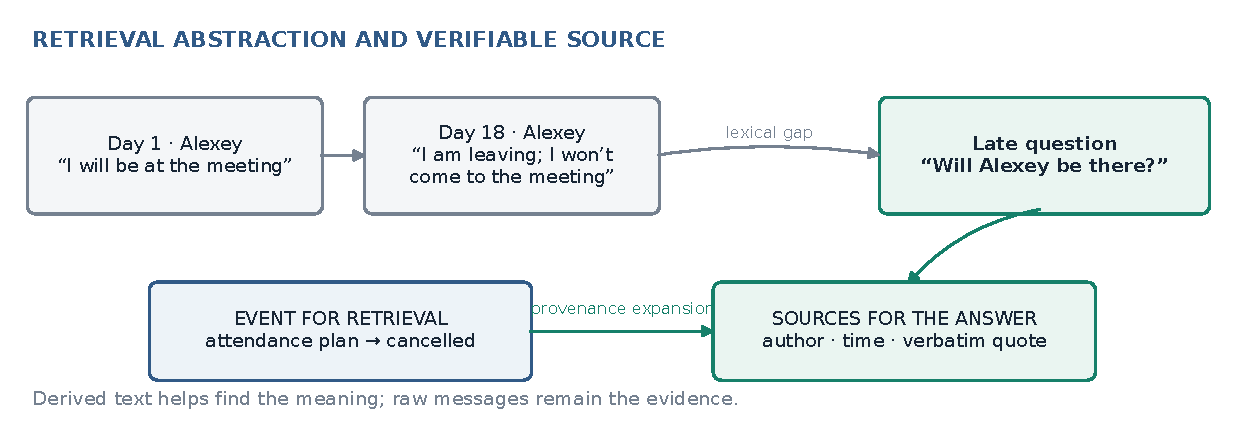
\includegraphics[width=\linewidth]{figures/concept.pdf}
\caption{Two-view memory: a normalized event serves as the semantic bridge, while
the answer is built from the returned primary messages. The example is
illustrative and is not part of any benchmark.}
\label{fig:concept}
\end{figure}

We propose to treat derived memory not as a new source of truth but as an
\emph{index over evidence}. In our implementation, \method{}, an event contains
(i) text optimized for semantic retrieval; (ii) a type, a viewpoint owner, a
subject and an observed time; (iii) an immutable set of source IDs and literal
quotes. Events compete with raw turns in a single vector top-$k$, and the selected
derived documents expand back into messages. Episodes are an optional layer: they
link revision, reaffirmation and augmentation, but do not replace events or their
sources.

The central question of this work: \emph{does an event index help find evidence
distributed across participants, messages and moments in time, while preserving
access to the original sources?} Questions about duration and changes of state are
a hard special case of this task. We answer in three steps: we measure the delivery
of annotated sources on all questions, test the temporal advantage with controls
for volume, order and query expansion, and determine what linking into episodes
and transfer to other benchmarks add.

\paragraph{Contributions.}
\begin{enumerate}
\item \textbf{Method.} An event index with addressable sources: the retrieval
description is separated from the immutable support, each event carries a
viewpoint owner, a subject, a time and \emph{source ID + verbatim quote} pairs, and
a retrieved event expands back into the original messages.
\item \textbf{Improved evidence delivery.} On all 2,400 EverMemBench questions the
event index raises the precision and recall of delivered gold sources relative to
a strong dense RAW baseline, while returning fewer unique sources and more gold
hits; the direction holds in all five projects and is supported on SocialMemBench.
\item \textbf{Separate evaluation of delivery and answers.} The full system reaches
47.16\% macro accuracy in an adapter evaluation of EverMemBench; the temporal
advantage of events persists after controls for budget, order and HyDE; paired
comparisons delimit the benefit: a mean accuracy gain from events and from linking
into episodes is not established, and transfer across the three benchmarks is
heterogeneous.
\end{enumerate}
Memory, runs and statistics are sealed, and every number in the paper is
recomputed offline (Appendix~\ref{app:reproduce}).

\section{Related work}

\paragraph{Agent memory and conversational tasks.}
Generative Agents combine an experience stream, retrieval and reflection
\citep{park2023}; MemGPT manages context tiers \citep{packer2023}. Mem0
consolidates facts \citep{chhikara2025mem0}, Zep/Graphiti uses a temporal graph
\citep{rasmussen2025zep}, A-MEM links notes \citep{xu2025amem}, Hindsight separates
facts, experience and beliefs \citep{latimer2025hindsight}, and HippoRAG implements
graph association \citep{gutierrez2024hipporag}. Unlike a general-purpose memory
manager, our evaluation focuses on multi-party conversation with stable
participant identifiers. LoCoMo and LongMemEval study multi-session memory
\citep{maharana2024,wu2024}; EverMemBench, GroupMemBench and SocialMemBench add,
respectively, long collaborative projects, reply structure and social attribution
\citep{hu2026,yang2026,owolabi2026}.

\paragraph{Closest retrieval representations.}
Dense X Retrieval indexes atomic self-contained propositions
\citep{chen2023densex}. RAPTOR builds a hierarchy of summaries; in collapsed-tree
mode original leaves and derived nodes are ranked together \citep{sarthi2024raptor}.
Self-contained statements and a joint pool of raw and derived documents are thus
known. \method{} carries them over to changing conversational states: an event
explicitly separates the author, the opinion owner and the subject, carries an
observed time and a per-fact \emph{source ID + verbatim quote} pair, and the source
address does not depend on the retrieval description or the episode version.
Experimentally, we compare this construction with our own strong RAW baseline and
separate the contributions of source delivery, context volume, order and episode
linking; the work contains no direct comparison with proposition retrieval or with
summaries carrying the same provenance (§\ref{sec:limits}).

\paragraph{Query expansion and verifiability.}
HyDE generates a hypothetical document for the query embedding \citep{gao2023hyde};
event memory normalizes the corpus in advance. We compare the two on Temporal
Duration with budget and order aligned. Like work on RAG and citation
\citep{lewis2020,gao2023}, we separate retrieval of support from answer quality: an
existing pointer does not prove the semantic correctness of a paraphrase.

\section{Problem statement}
\label{sec:problem}

Let $M=(m_1,\ldots,m_n)$ be the history of a single bounded conversation space. A
message $m_i=(id_i,g_i,a_i,t_i,x_i)$ contains the space, the author, the time and
the text. A builder $B$ receives only $M$ and creates memory $\mathcal{D}$ before QA
opens. For a query $q$, retrieval selects documents $R_k(q,\mathcal{D})$, after
which the generator answers from the expanded context $C_q$.

We distinguish three properties:
\begin{enumerate}
\item \textbf{pointer integrity}: the source ID exists, and the quote is literally
contained in it;
\item \textbf{semantic support}: the source text actually entails the derived
description;
\item \textbf{answer correctness}: the generator used the delivered context
correctly.
\end{enumerate}
A mechanical check guarantees only the first. The second requires an entailment
or human audit; the third is measured by benchmark scoring.

\section{Method}
\label{sec:method}

\subsection{The immutable event}

An event has the form
\[
e=(z,o,s,k,r,\tau,P,L),
\]
where $z$ is the self-contained index text, $o$ the viewpoint owner, $s$ the
subject, $k$ the event type, $r$ the temporal mode, $\tau$ the observed time, $P$
the evidence and $L$ the local context. Evidence consists of pairs
$(id_i, quote_i)$; time is derived from the real timestamps of the sources.

Separating $o$ from $s$ lets ``A called B unreliable'' be represented as A's
opinion about B rather than as an unconditional fact about B; the correctness of
these fields depends on extraction quality. The types cover state, opinion,
decision, commitment, relationship, exception and the category \texttt{other}. A
conversational reaction without long-term content may produce no event; a cap of at
most two events per turn applies.

\needspace{16\baselineskip}
\paragraph{Example.}
An illustrative fragment of one working session, not from a benchmark:
\begin{quote}\small
10:02, Marina: ``We move the release to Friday~--- Oleg's payment module isn't done.''\\
10:05, Oleg: ``I'll finish it by tonight.''\\
18:40, Oleg: ``Done, ready to ship.''
\end{quote}
A week later the question is asked: ``Who held up the release, and did they finish
their part?'' The answer is contained in the 18:40 message, but it mentions neither
the release, nor the payment module, nor the person concerned: its link to the
question exists only through neighbouring messages. The schema admits two events:
\begin{itemize}
\item $e_1$: $z$~= ``Marina tied moving the release to Friday to Oleg's unfinished
payment module''; $o$~= Marina, $s$~= Oleg, $\tau$~= 10:02; $P$: (10:02, ``Oleg's
payment module isn't done'').
\item $e_2$: $z$~= ``Oleg reported that he finished the payment module''; $o$~= Oleg,
$s$~= payment module, $\tau$~= 18:40; $P$: (18:40, ``Done, ready to ship''); the
messages at 10:02 and 10:05 are in $L$ as context resolving ``done''.
\end{itemize}
The index text of $e_2$ makes the short confirmation retrievable by the words of the
question, and the quote points to the original message. The same example shows
the boundary of this guarantee. The quote confirms that the message exists and was
written by Oleg at 18:40, but it does not confirm the interpretation ``finished the
payment module'': that rests on messages in $L$. Only the sources in $P$ are
returned to the generator together with the event; messages in $L$ reach the
context only if retrieval finds them independently. The explanatory message at
10:02 is therefore better included in $P$, and the literal quote check does not
ensure this: it is semantic support (property~2 in §\ref{sec:problem}), not pointer
integrity. The fields play different roles: $o$ distinguishes Marina's statement
\emph{about} Oleg from Oleg's own message, $s$ specifies whom or what the fact is
about, and $\tau$ separates the state ``not done'' from the later ``done''. The
example illustrates the role of the schema fields; measured effects are reported
in §\ref{sec:delivery}--\ref{sec:episodes}.

\subsection{Query-independent extraction and validation}

The history is split along benchmark sessions: in EverMemBench by day and group;
in GroupMemBench by channel/phase with blocks of up to 40 messages. Forced
structured output permits an empty list. A deterministic validator then removes
invented IDs, missing quotes, content-free values and invalid enums. Local context
can help resolve a pronoun, but does not automatically become evidence.

\subsection{Optional versioned episodes}

An episode $E_j=((e_1,\rho_1),\ldots,(e_t,\rho_t))$ is an append-only line where each operation $\rho$ is one of \texttt{create},
\texttt{revise}, \texttt{reaffirm} or \texttt{augment}.
For a new event, candidates are searched only within the conversation network. The
score is
\[
S(e,E)=0.6\cos(\phi(z_e),\phi(A_E))+0.4\cos(\phi(z_e),\phi(z_{last(E)})).
\]
Here $A_E$ is the concatenation of the last five events, $z_{last(E)}$ the last
event, and $\phi$ a local MiniLM embedding for linking. The three best episodes go
to an LLM resolver. With an empty pool, an invalid choice or confidence below 0.5,
a new episode is created; this is a safeguard branch, not an additional search.
Answer retrieval uses a separate embedding in the benchmark adapter. The index
keeps a hot view of the last five events, while cold events and evidence are not
deleted. We assume that a false split is cheaper than a false merge: split events
can still reach retrieval independently, whereas an erroneous merge can bring
extraneous sources into later requests; the frequencies of both errors were not
measured.

\subsection{Unified retrieval and provenance expansion}

A raw turn and a derived document share a common interface
\[
d=(id,\ kind,\ index\_text,\ render\_text,\ source\_ids).
\]
The question vector is compared against a single pool; the top-$10$ can contain
both kinds. After ranking, each event/episode expands into unique raw turns. The
generator sees the derived text as a navigational hint and the dated,
speaker-grounded sources as the basis of the answer.

Derived memory passes the same relevance criterion as raw history; static user
profiles are not added.

\FloatBarrier
\begin{figure}[t]
\centering
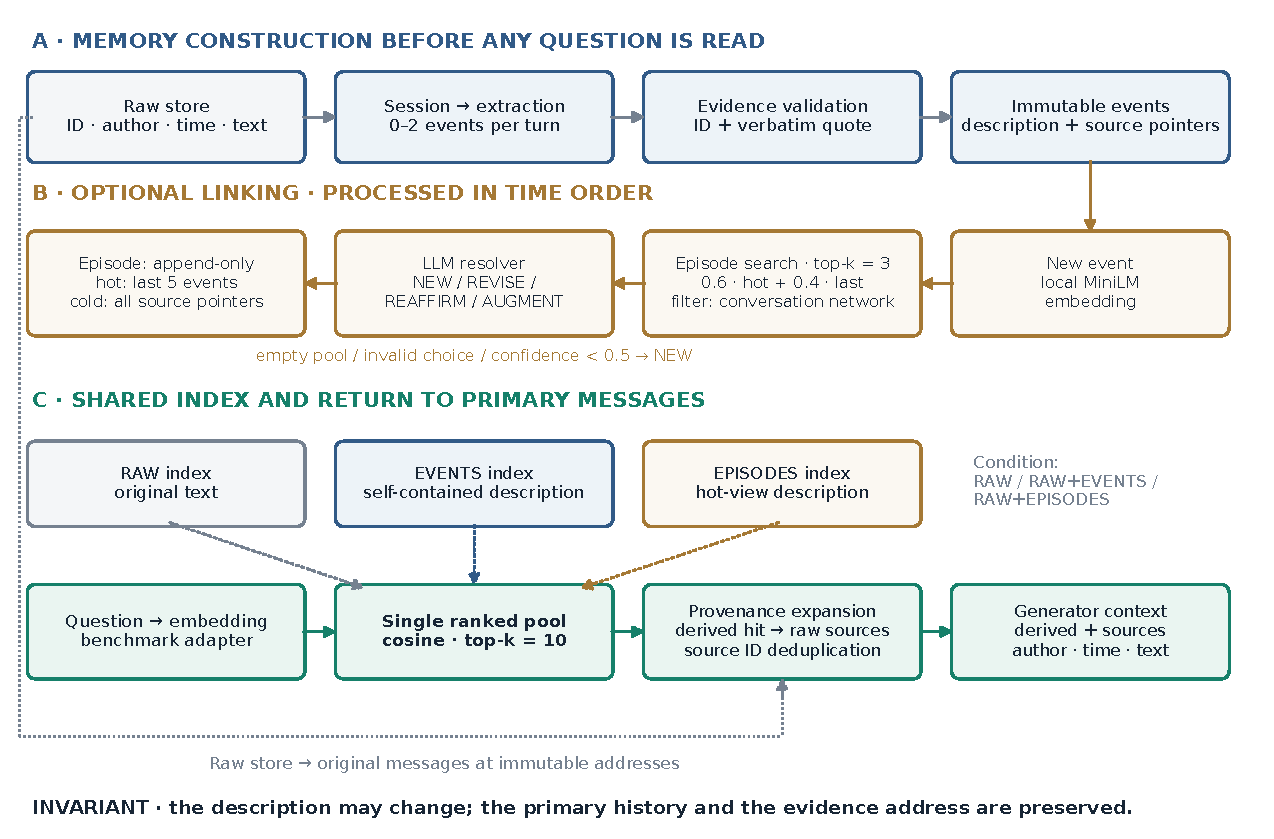
\includegraphics[width=\linewidth]{figures/architecture.pdf}
\caption{The full architecture. Memory is built query-independently and sealed
before QA. In the main variant raw turns and episodes are ranked jointly; in the
ablation, episodes are replaced by separate events. A derived hit always expands
into raw sources.}
\label{fig:architecture}
\end{figure}

\section{Experimental protocol}

\subsection{Data and conditions}

\begin{table}[ht]
\centering\small
\begin{tabularx}{\linewidth}{lrrX}
\toprule
Benchmark & QA & Spaces & Main test\\
\midrule
EverMemBench & 2,400 & 5 projects & 9 task types; temporal controls\\
SocialMemBench & 1,031 & 43 networks & social attribution, norms, updates\\
GroupMemBench & 745 & 4 domains & reply structure, implicit, multi-hop\\
\bottomrule
\end{tabularx}
\caption{External datasets used. For GroupMemBench, 102 initially empty generation
outputs were restored by a separate sealed amendment; the original protocol result
is retained.}
\label{tab:data}
\end{table}

The main paired baseline is a strong dense \raw{}, not a weak keyword-only search.
The \events{} and \episodes{} conditions add derived documents to the same
top-$10$. For Temporal Duration the token budget and chronological order are also
controlled; in the reordering controls the set of sources is fixed within each
condition, but not between RAW and EVENTS. HyDE generates a hypothetical document
only for the query embedding and returns the same raw documents. All variants use
the same official answer/judge prompts inside the corresponding benchmark adapter.

EverMemBench uses GPT-4.1-mini for answering, Gemini-3-Flash-preview as the
open-answer judge, text-embedding-3-large for retrieval and gpt-4o-mini-2024-07-18
for memory construction. The answer and judge models, their prompts and the exact
multiple-choice scoring are taken from the official harness; providers are pinned
(OpenAI and Google AI Studio respectively) with fallbacks disabled~--- this aligns
the evaluation models, but not every other component of other systems. EverMemBench
answers and judging use \texttt{temperature}${}=0$. SocialMemBench follows the
GPT-4o-mini official-compatible harness. GroupMemBench uses the GPT-5 of the
official run; the provider's model version was not pinned by date, so byte-level
reproduction of these numbers is not guaranteed. Comparisons across benchmarks are
not interpreted as comparisons of models.

\subsection{Metrics and statistics}
\label{sec:stats}

We report micro accuracy, macro accuracy over official question types, and paired
differences between conditions. For a question $q$ let $U_q$ be the set of unique
expanded sources and $G_q$ the gold anchors released by the benchmark:
\[
P_q=\frac{|U_q\cap G_q|}{|U_q|},\qquad
R_q=\frac{|U_q\cap G_q|}{|G_q|}.
\]
With an empty $U_q$ precision is zero; with an empty $G_q$ the scorer sets recall to
one; in the verified Ever questions $G_q$ is non-empty. Tables report \emph{means of
per-question ratios}, not the ratio of total hits to total sources. These metrics
measure the delivery of annotated support, not entailment, context sufficiency or
the correctness of user-facing citations.

95\% CIs for Ever and Group come from a paired question bootstrap; for transfer to
Social, 43 conversation networks are additionally resampled. Accuracy is compared
with exact McNemar. Question-level intervals describe the studied set: its
questions are not equivalent to independent projects. For evidence we therefore
also report the effect per Ever project and a leave-one-project-out sensitivity
(Appendix~\ref{app:verification}).

Temporal Duration was selected after inspecting the full breakdown, so its analysis
is marked exploratory; the correction for the choice of category is given in
§\ref{sec:temporal}. Protocols, revisions and artifact sealing are in the appendix.

\section{Results: system level and paired comparisons}

Two questions are separated here. How strong the full system is in absolute terms
is shown by a descriptive comparison with published rows (§\ref{sec:external}).
What event memory itself adds is shown only by paired comparisons with our RAW on
the same questions (§\ref{sec:paired}) and by the controls in §\ref{sec:mech}. The
first answer characterizes the level the system achieves, the second the
contribution of the event layer.

\subsection{Comparison with published systems}
\label{sec:external}

\paragraph{EverMemBench.}
\begin{figure}[t]
\centering
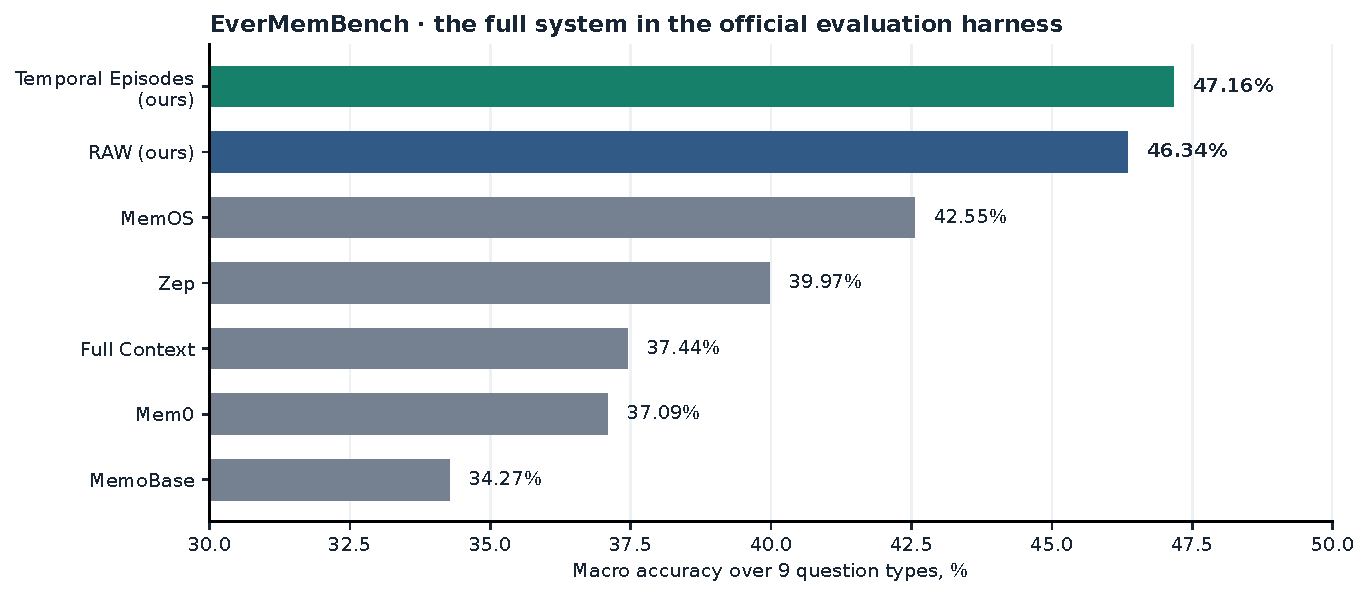
\includegraphics[width=.96\linewidth]{figures/ever_leaderboard.pdf}
\caption{Macro accuracy over the nine EverMemBench categories with the GPT-4.1-mini
answer backbone. Published results are from the benchmark paper \citep{hu2026}; our
rows come from an adapter evaluation on top of the official harness. The comparison
is descriptive: not an official leaderboard submission and not a paired test
against other systems.}
\label{fig:leaderboard}
\end{figure}

The full \episodes{} system reaches \textbf{47.16\% macro}, and \raw{} 46.34\%. Our
adapter result is above the values reported by \citet{hu2026} with the same answer
backbone: MemOS 42.55\%, Zep 39.97\%, Mem0 37.09\%, Full Context 37.44\% and MemoBase
34.27\%. The gap to the best published memory system is 4.61 pp.

\begin{table}[ht]
\centering\small
\begin{tabular}{@{}lrrrrr@{}}
\toprule
System & Macro & Multi-hop & Temporal & Update & Style\\
\midrule
\episodes{} (ours) & 47.16 & 13.25 & 20.00 & 47.39 & 38.07\\
\events{} (ours) & 46.82 & 13.25 & 16.33 & 47.01 & 33.52\\
\raw{} (ours) & 46.34 & 12.85 & 12.33 & 46.27 & 30.11\\
\midrule
MemOS & 42.55 & 18.88 & 15.67 & 45.15 & 28.98\\
Zep & 39.97 & 8.03 & 13.00 & 43.66 & 26.70\\
Mem0 & 37.09 & 11.24 & 6.33 & 51.87 & 22.73\\
MemoBase & 34.27 & 12.85 & 18.00 & 30.60 & 17.05\\
\bottomrule
\end{tabular}
\caption{Absolute EverMemBench level, accuracy in percent; answer model GPT-4.1-mini.
Other systems: Table 4 of arXiv:2602.01313v3 \citep{hu2026}; our rows: full runs
without token/order controls. Macro averages all nine types; the other columns show
four diagnostic slices. There is no paired statistical test between the blocks.}
\label{tab:ever-external}
\end{table}

On Temporal our \episodes{} reaches 20.00\%, against 6.33--18.00\% for the published
memory rows. The per-category profile is heterogeneous: MemOS is higher on
Multi-hop, Mem0 on Update.

The comparison records the level achieved by the full adapter; other systems were
not rerun on a single infrastructure. Our own strong \raw{} (46.34\%) shows that most
of this level comes from retrieval and the answer model, and the added contribution
of memory is measured pairwise in §\ref{sec:paired}.

\paragraph{SocialMemBench.}
On SocialMemBench the full system reaches MeanQ .368 (\episodes{}) and .358
(\raw{}): practically at the level of the published full-context .369 and above the
listed benchmark memory rows (best Subject-Mem .321).

\begin{table}[ht]
\centering\small
\begin{tabular}{@{}lrrrrr@{}}
\toprule
System & MeanQ & Attribution & Decisions & ToM & State change\\
\midrule
\episodes{} (ours) & .368 & .863 & .691 & .262 & .259\\
\raw{} (ours) & .358 & .825 & .716 & .251 & .233\\
\midrule
Subject-Mem & .321 & .780 & .610 & .240 & .220\\
SMG & .213 & .440 & .690 & .110 & .100\\
Graphiti & .178 & .460 & .610 & .050 & .070\\
LangMem & .162 & .390 & .560 & .060 & .090\\
Mem0 & .143 & .310 & .570 & .050 & .070\\
Cognee & .120 & .250 & .590 & .100 & .010\\
\bottomrule
\end{tabular}
\caption{SocialMemBench: question-weighted scores (0--1), not binary accuracy. All
rows use GPT-4o-mini. Other systems: Table 4 of \citep{owolabi2026}; ours: frozen
official-v1 harness. Columns correspond to Q4/AP, Q2/GD, Q5/TM and Q8/TS. The
comparison with external rows is descriptive.}
\label{tab:social-external}
\end{table}

The comparison exposes different demands on memory: the adapter achieves high
attribution (.863 for \episodes{}), while theory of mind and reconstructing state
changes remain hard even with preserved sources. On group decisions \episodes{} trail
our \raw{} (.691 versus .716), so the high overall level reflects the whole adapter,
not linking alone.

\paragraph{GroupMemBench.}
On GroupMemBench external results also depend on the task type
(Appendix~\ref{app:group-external}). For example, published Hindsight reaches
54.94\% on Temporal but 17.76\% on Update; our EPISODES reaches 36.42\% and 23.36\%
respectively. Published BM25 reaches 54.94\% on Temporal and 25.23\% on Update:
comparing only against heavy memory systems would hide a strong simple
alternative.

\subsection{Paired comparisons within our conditions}
\label{sec:paired}

\paragraph{EverMemBench.}
\begin{table}[ht]
\centering\small
\begin{tabular}{lrrrr}
\toprule
Condition & Micro & Macro & Evid. recall & Evid. precision\\
\midrule
\raw{} & 49.46 & 46.34 & 8.08 & 21.29\\
\events{} & 49.83 & 46.82 & 8.71 & \textbf{24.50}\\
\episodes{} & \textbf{50.21} & \textbf{47.16} & \textbf{10.75} & 22.45\\
\bottomrule
\end{tabular}
\caption{EverMemBench, all 2,400 QA, percent. Macro is the mean over the nine
official question types; micro is over individual QA.}
\label{tab:ever-main}
\end{table}

At the micro level \episodes{} improve 49.46\%$\rightarrow$50.21\%: $+0.75\pp$, 95\% CI
$[-0.5;+2.0]$, $p=.256$. \events{} reach 49.83\%: $+0.38\pp$, CI $[-0.8;+1.6]$,
$p=.589$. Both intervals include zero: a mean accuracy gain in the paired comparison
is not established.

\paragraph{Transfer across benchmarks.}
\begin{figure}[ht]
\centering
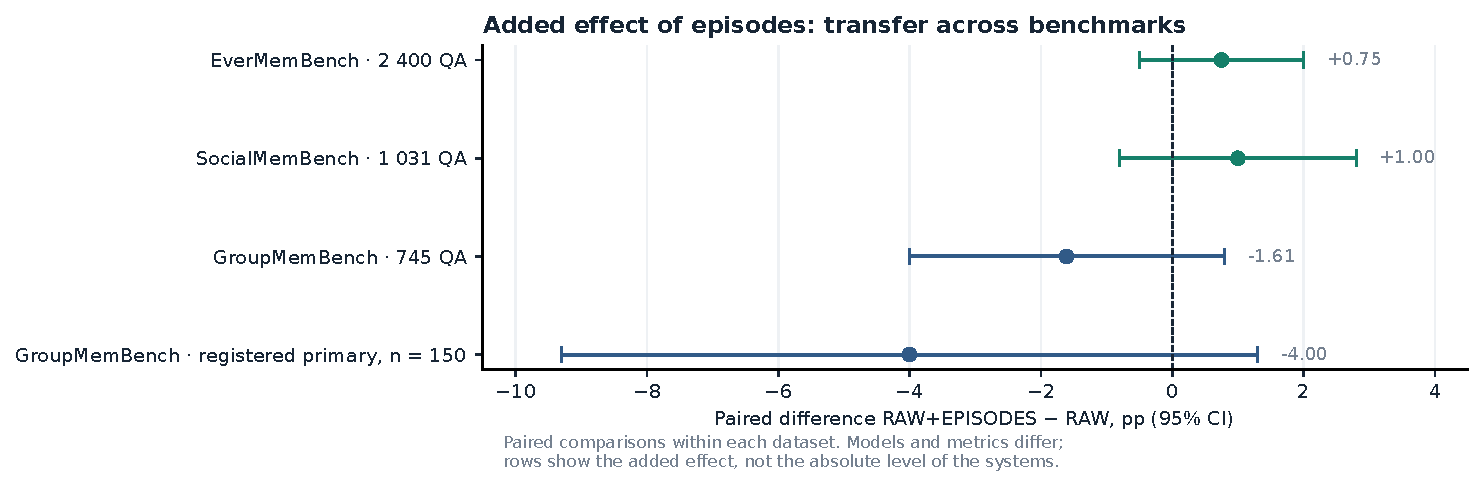
\includegraphics[width=.92\linewidth]{figures/transfer.pdf}
\caption{Paired differences \episodes{}$-$\raw{} within each dataset with question- or
network-bootstrap 95\% CIs. Only paired differences are shown: the metric (accuracy
versus MeanQ), protocols and answer models differ across the three datasets. Group
is shown after the targeted repair of empty generations; its separately registered
temporal/update endpoint ($n=150$ of 745) is shown as its own row. No interval
excludes zero.}
\label{fig:transfer}
\end{figure}

On SocialMemBench the paired difference \episodes{}$-$\raw{} is $+0.010$ MeanQ,
network-bootstrap 95\% CI $[-.008;+.028]$: a mean MeanQ gain is not established.

At the level of delivery, Social supports the EverMemBench direction. The precision
of delivered sources rises relative to \raw{} for flat memory ($+0.90\pp$,
network-bootstrap 95\% CI $[+0.66;+1.19]$), versioned ($+0.86\pp$, $[+0.61;+1.16]$)
and episodes ($+0.34\pp$, $[+0.15;+0.54]$); all three intervals exclude zero. The
result comes from a different conversation structure and a different answer model.
The memory schemas are not identical: flat and versioned were built by an earlier
extractor, and the base evidence recall on Social (67.5\%) is substantially higher
than on Ever, so absolute effect sizes are not comparable across datasets.

On GroupMemBench transfer is heterogeneous. On the pre-registered Group primary
(Finance and Technology; knowledge update and temporal; $n=150$), after restoring empty
answers, \raw{} reaches 37.3\% and \episodes{} 33.3\%: $\Delta=-4.0\pp$, CI
$[-9.3;+1.3]$; over all 745 QA, 43.1\% versus 41.5\%, $\Delta=-1.6\pp$, CI
$[-4.0;+0.8]$. The direction is negative and persists after the repair; the
intervals include zero. Details of the 102 restored generations and of the original
protocol result are in Appendix~\ref{app:repair}.

\section{The event representation: delivery and temporal answers}
\label{sec:mech}

We first examine the direct change in retrieved sources, then its link to answer
quality. This order evaluates the retrieval layer separately from the overall level
of the answer model.

\subsection{Evidence delivery: the main result}
\label{sec:delivery}

We compare, pairwise and per question, the share of delivered gold sources (recall)
and their density in the context (precision) on all 2,400 questions, without slice
selection.

\begin{figure}[t]
\centering
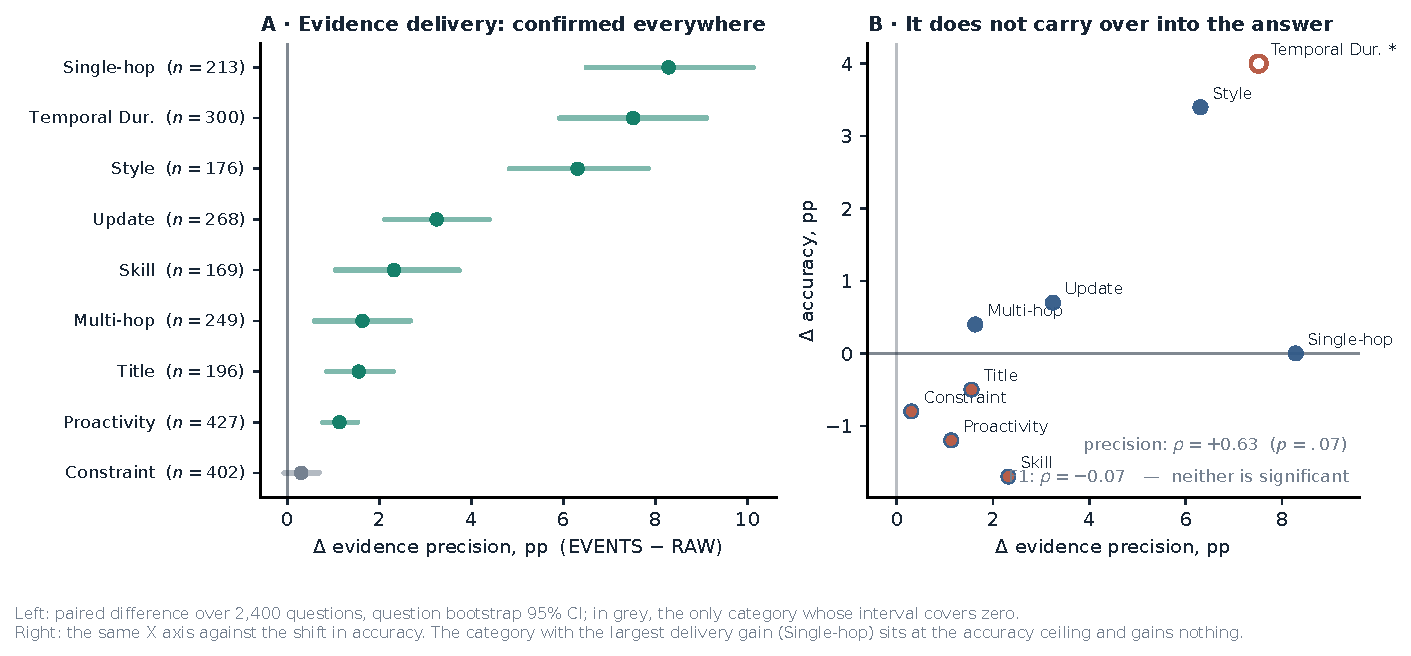
\includegraphics[width=\linewidth]{figures/dissociation.pdf}
\caption{Evidence delivery and accuracy. \textbf{A}: paired difference in evidence
precision \events{}$-$\raw{} over the nine official categories, all 2,400 questions,
question bootstrap 95\% CI; the sign is positive everywhere, and the interval
includes zero only for Constraint. \textbf{B}: the same axis against the shift in
accuracy; the asterisk marks the post hoc discovery slice. The category with the
largest delivery gain (Single-hop, $+8.28\pp$) sits at an accuracy ceiling of 89.7\%
and gains nothing. The points describe heterogeneity across categories, not a
causal link between delivery and answers.}
\label{fig:dissociation}
\end{figure}

\begin{table}[ht]
\centering\small
\begin{tabular}{lrrr}
\toprule
Condition & Sources & Gold hits & Evid. precision\\
\midrule
\raw{}      & 10.00 & 2.129 & 21.29\\
\events{}   & \textbf{9.47} & \textbf{2.245} & \textbf{24.50}\\
\episodes{} & 12.38 & 2.795 & 22.45\\
\bottomrule
\end{tabular}
\caption{EverMemBench, all 2,400 QA: how many unique sources entered the context, how
many of them were gold anchors, and what share of the context was gold. On average
\events{} have fewer sources and more gold hits than \raw{}.}
\label{tab:delivery}
\end{table}

\events{}$-$\raw{}, paired: precision $+3.21\pp$ (95\% CI $[+2.84;+3.59]$, 855
questions better against 255 worse), recall $+0.64\pp$ ($[+0.48;+0.80]$). The sign of
the precision gain is positive in all nine official categories, and the CI excludes
zero in eight of nine (Table~\ref{tab:evid-cats}). The effect does not rest on a
single project: the gain is positive in each of the five EverMemBench projects, and
leaving out any one project keeps it within 3.11--3.39\pp{}
(Appendix~\ref{app:verification}). The event index thus brings more annotated support
into a fixed top-10.

\paragraph{The precision gain is not reducible to fewer returned sources.}
Precision could rise simply because fewer sources are returned. The data show
otherwise: \events{} return on average 9.47 sources against 10.00 for \raw{}, and
\emph{on no question} more, yet find more gold hits~--- $2.245$ against $2.129$ per
question, a delta of $+0.117$ (CI $[+0.083;+0.151]$); on 449 questions gold hits are
strictly higher without an increase in the number of sources. The event index
improves the selection of support rather than merely shortening the list. In tokens
the context is longer: the derived event text yields on average 1177 versus 1054
\texttt{o200k\_base} tokens (recomputed offline from the sealed retrieval), so the
role of volume in the temporal result is tested by a separate token control
(§\ref{sec:temporal}). \episodes{} behave differently: they raise recall together with
volume ($+2.68\pp$ recall at $+2.4$ sources), and their precision grows less
($+1.16\pp$).

\paragraph{Query-side expansion does not reproduce this.}
On Temporal Duration, at an approximately equal budget and the same order, matched
HyDE obtains a similar recall~--- 20.7\% against 19.7\% for \events{} (difference
EVENTS$-$HyDE $-1.01\pp$, CI $[-2.20;+0.17]$) --- but a markedly sparser context: the
precision of \events{} is higher by $+6.68\pp$ (CI $[+5.06;+8.27]$). Against
token-matched \raw{}, HyDE raises precision by $+1.18\pp$ and recall by $+1.61\pp$.
Query expansion and corpus normalization produce different delivery profiles: at a
similar recall the event index delivers denser support. Dominance of \events{} on
both coordinates is not established: their recall is slightly lower, and a
non-significant difference does not mean equivalence.

\paragraph{Why low recall is compatible with high accuracy.}
Ever gold annotation contains a median of 27 sources per question (interquartile
range 21--37; maximum 96), while RAW returns ten. This sets a low completeness
relative to the whole reference set. In RAW, 316 of 2,400 questions received a
correct verdict without a single delivered gold anchor; in EVENTS, 312. Gold
intersection and accuracy measure different properties of the system; the
sufficiency of evidence for the answer was not evaluated separately.

\subsection{Temporal Duration: the advantage after controls}
\label{sec:temporal}

In the original Temporal Duration breakdown RAW reaches 12.3\% and EPISODES 20.0\%.
But episodes expand into several messages: on average 17.4 sources against ten for
RAW. We therefore successively tested raw-context expansion, chronological order,
separate events instead of linked episodes, and HyDE on the query side.

Token matching uses the token count of the expanded EPISODES context as the target
budget and selects the closest prefix of ranked documents without truncating
messages; this aligns budgets, it does not make them byte-identical. Matched HyDE
targets the EVENTS context. Chrono controls change only the order of already
selected blocks, keeping their sources. Mean chrono context sizes: RAW 2458, EVENTS
2456, HyDE 2451 tokens. The per-question absolute difference between EVENTS and RAW
has a median of 35 tokens (1.48\%), a 95th percentile of 97 (4.60\%) and a maximum of
139 (11.46\%). Full deviations and their computation rules are in
Appendix~\ref{app:tokens}.

\begin{figure}[t]
\centering
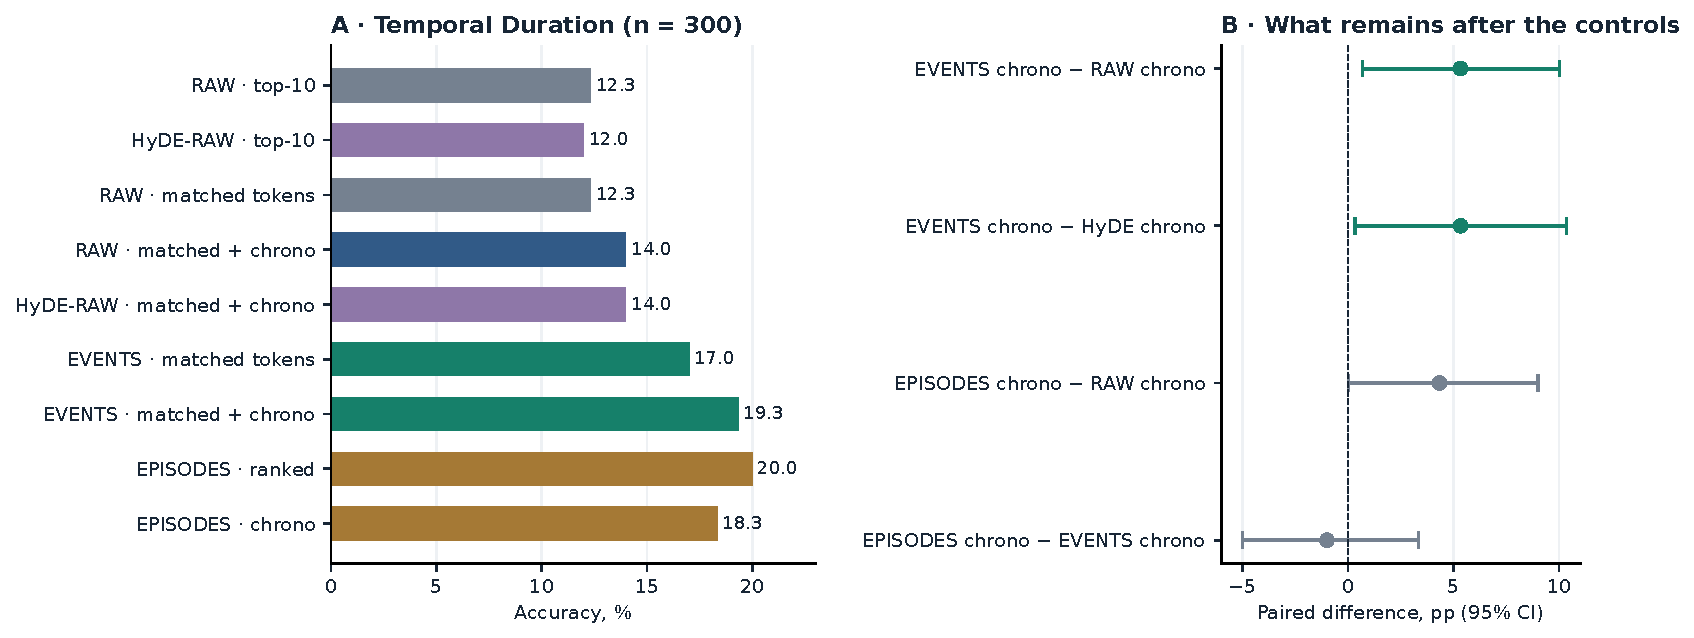
\includegraphics[width=\linewidth]{figures/temporal_controls.pdf}
\caption{Controls for representation, volume and order on exploratory Temporal
Duration. EVENTS chrono keep the observed advantage over RAW and HyDE at an
approximately equal token budget and the same order; EPISODES do not exceed EVENTS.
Intervals are question bootstrap 95\%.}
\label{fig:controls}
\end{figure}

\begin{table}[ht]
\centering\small
\begin{tabular}{lrrr}
\toprule
Condition & Accuracy & Evid. recall & Evid. precision\\
\midrule
RAW top-10 & 12.3 & 12.7 & 29.6\\
HyDE-RAW top-10 & 12.0 & 14.1 & 32.4\\
RAW count-matched & 13.3 & 16.6 & 25.1\\
RAW token-matched & 12.3 & 19.1 & 21.5\\
RAW token-matched chrono & 14.0 & 19.1 & 21.5\\
HyDE-RAW token-matched chrono & 14.0 & \textbf{20.7} & 22.6\\
EVENTS token-matched & 17.0 & 19.7 & 29.3\\
EVENTS token-matched chrono & 19.3 & 19.7 & 29.3\\
EPISODES ranked & \textbf{20.0} & \textbf{20.5} & \textbf{31.1}\\
EPISODES chrono & 18.3 & \textbf{20.5} & \textbf{31.1}\\
\bottomrule
\end{tabular}
\caption{Temporal Duration, $n=300$, percent. Precision and recall are means of
per-question ratios after source expansion.}
\label{tab:controls}
\end{table}

At an approximately equal token budget and the same order, \events{} reach 19.3\%
against 14.0\% for \raw{}: $+5.33\pp$, 95\% CI $[+0.67;+10.0]$, nominal $p=.0402$.
Matched HyDE also obtains 14.0\%; the difference \events{}$-$HyDE is $+5.33\pp$, CI
$[+0.33;+10.33]$, nominal $p=.0479$ (37 wins against 21 losses). The direction is
positive in all five projects. Outside Temporal Duration, on 2,100 questions,
\events{} give $-0.14\pp$ (CI $[-1.33;+1.10]$, $p=.877$): the advantage is concentrated
in this slice rather than spread over all tasks.

The advantage comes with a characteristic delivery profile. Events combine the
recall of expanded RAW (19.7\% against 19.1\%) with the precision of RAW top-10
(29.3\% against 29.6\%), whereas HyDE raises recall to 20.7\% at 22.6\% precision and
14.0\% accuracy. This profile is consistent with the temporal advantage; the link
between delivery and answers is tested in §\ref{sec:frontier}.

\paragraph{Status of the temporal signal.}
The slice was selected post hoc from nine categories. With a conservative Bonferroni
correction the nominal $p=.0402$ and $.0479$ become about $.36$ and $.43$; with five
projects the two-sided exact sign-flip test used cannot reach $p<.05$ (minimum
$.0625$). Fixing the matched-HyDE endpoint in advance covers the analysis but not the
choice of slice. The temporal result is thus a substantive exploratory signal,
robust to controls for budget, order and HyDE, but not a confirmed effect.

\subsection{Link between source delivery and answer quality}
\label{sec:frontier}

Before computing it, we recorded a rule for an offline check: outside Temporal
Duration, split the questions by whether \events{} or \raw{} dominate on recall and
precision, and compare the direction of accuracy. In the stratum where \events{}
deliver strictly better support ($n=650$), accuracy changes by $+0.77\pp$ (CI
$[-1.85;+3.54]$); where \raw{} dominates ($n=209$), by $-2.39\pp$ ($[-6.70;+2.39]$).
The directions match the hypothesis, but the pre-registered confirmation criterion
is not met (Appendix~\ref{app:frontier}).

This result separates what is established from what is open. The improvement in
delivery is measured directly and consistently; its transfer to accuracy is not
confirmed on the available samples. Evaluating the two endpoints separately shows
which benefit the event layer already provides and which remains to be established.
The check was run on a previously studied set, does not establish a causal mechanism
and does not rule out an effect of delivery on answers: the interval in the stratum
with better delivery also admits a noticeable positive effect.

\subsection{What episodes add over events}
\label{sec:episodes}

In symmetric controls \episodes{} chrono obtain 18.3\% and \events{} chrono 19.3\%: a
difference of $-1.0\pp$, CI $[-5.0;+3.33]$, $p=.755$. In the previously sealed
comparison of ranked episodes (20.0\%) and events chrono (19.3\%), the difference was
$+0.67\pp$, $p=.888$. An added mean accuracy gain from linking is not established.

Linking changes the delivery profile (§\ref{sec:delivery}) and keeps an inspectable
chronology of revisions, reaffirmations and augmentations with access to earlier
evidence. For retrieval in the studied scenario, separate events are the simpler
basis: split events reach the context independently through ordinary ranking.

\section{Efficiency and engineering properties}

\subsection{Cost and latency}

The full EverMemBench experiment recorded 26,413 API calls and an upper list-price
estimate of \$8.88. Of this, memory construction with gpt-4o-mini costs \$4.76,
embeddings \$0.46, answers \$3.12 and the judge \$0.55. These figures refer to a
research run with caches and are not a production TCO.

The total covers both conditions, repeats and answer scoring, not only \episodes{}
indexing, so the comparison with other systems below uses memory construction cost
on GroupMemBench. The serialized episode snapshot occupies 12.77 MB; a full
operational run together with the embedding cache is about 2.2 GB.

\begin{figure}[ht]
\centering
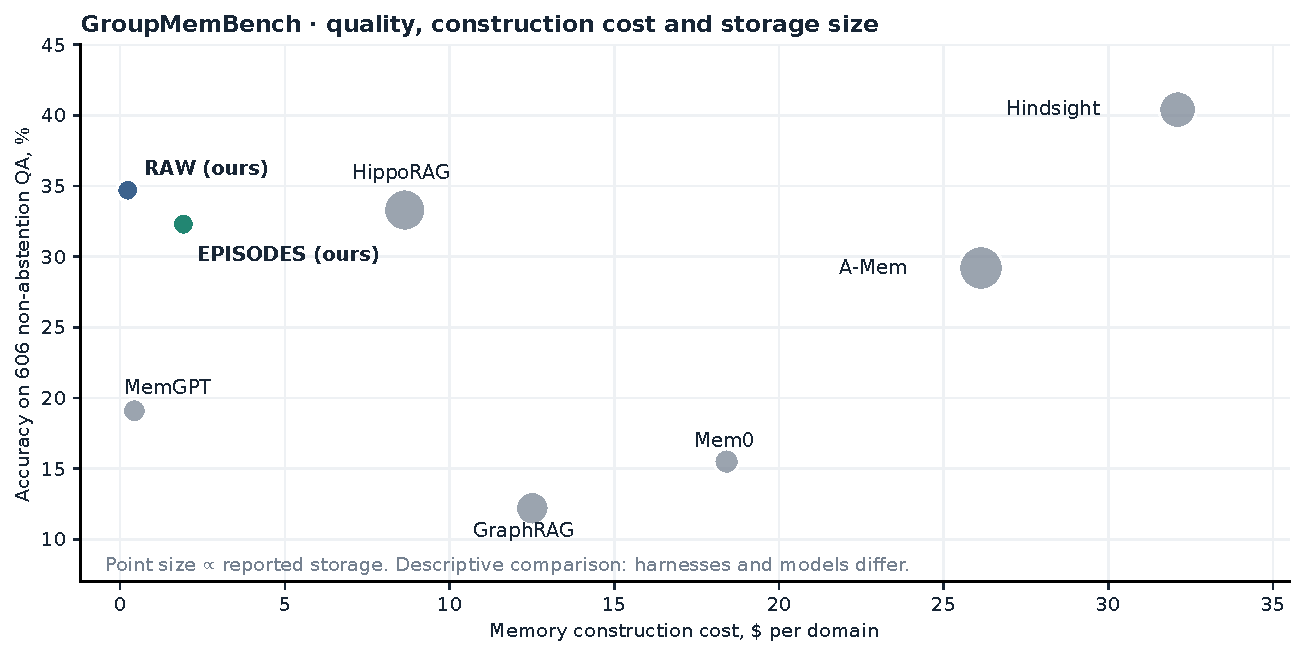
\includegraphics[width=.94\linewidth]{figures/efficiency.pdf}
\caption{A descriptive GroupMemBench efficiency landscape on the shared sample of 606
QA, from the values of the benchmark paper and of our adapter. Point size encodes
reported storage. Our points use the repaired amendment; cost definitions and
backends differ, so the plot describes an engineering trade-off, not a controlled
comparison of cost at equal quality.}
\label{fig:efficiency}
\end{figure}

\begin{table}[ht]
\centering
\small
\begin{tabular}{@{}lrrr@{}}
\toprule
System & Accuracy, \% & Ingestion, \$/domain & Storage, GB \\
\midrule
Hindsight & 40.4 & 32.10 & 4.25 \\
\textbf{\raw{} (ours)} & \textbf{34.7} & \textbf{0.23} & \textbf{0.37} \\
HippoRAG & 33.3 & 8.64 & 5.76 \\
\textbf{\episodes{} (ours)} & \textbf{32.3} & \textbf{1.92} & \textbf{0.41} \\
A-Mem & 29.2 & 26.13 & 6.60 \\
MemGPT & 19.1 & 0.43 & 0.69 \\
Mem0 & 15.5 & 18.41 & 0.99 \\
GraphRAG & 12.2 & 12.51 & 3.00 \\
\bottomrule
\end{tabular}
\caption{Explicit values for Figure~\ref{fig:efficiency}. Accuracy is an aggregate over
the five non-abstention task types of GroupMemBench (606 QA): for published systems it
is recomputed from per-type percentages (Appendix~\ref{app:group-external}), for ours it
is computed from the repaired results. It is a comparison of aggregates, not a single
run of all systems. Ingestion cost and storage come from the corresponding benchmark
reports. Our accuracies are recomputed after the targeted repair; the cost of the
repair answers is not included in ingestion. Backends, harnesses and storage
definitions differ, so the comparison is descriptive.}
\label{tab:efficiency}
\end{table}

On this shared sample Hindsight reaches 40.4\% at a reported ingestion of
\$32.10/domain and 4.25 GB; HippoRAG 33.3\%, \$8.64 and 5.76 GB; our \raw{} 34.7\%,
\$0.23 and 0.37 GB; \episodes{} 32.3\%, \$1.92 and 0.41 GB. The system is economical
relative to heavy structural solutions, but Hindsight is more accurate. Because the
harness components differ, this is context, not a controlled causal estimate of cost.

The adapter reaches accuracy at the level of HippoRAG without a large graph/database
backend: by the published values, Hindsight's construction costs about 16.7 times as
much as our \episodes{}, and its storage is 10.4 times larger; for HippoRAG these ratios
are 4.5 and 14.0. These are ratios of reported costs and sizes, not measurements of
RAM consumption on an identical workload.

\paragraph{What is known about speed.}
On 2,400 EverMemBench questions local ranking takes on average 11.59 ms for RAW and
13.70 ms for EPISODES: an extra 2.11 ms, about 18\%. The corresponding p95 values are
12.70 and 15.04 ms; network and generation are not included. The benchmark tables
used contain no comparable measurement of end-to-end query latency for other memory
systems, so speed is not compared with other systems; the duration of a full run also
depends on API latency, the number of workers, retries and rate limits.

\subsection{Engineering implications}
Memory construction is paid before any questions; retrieval does not call the linker
again. The hot view bounds the size of an indexed episode, while the cold history keeps
all evidence pointers. The retrieval description can therefore be corrected without
deleting the primary history. Sealing inputs and caching make it possible to separate
a change of method from repeated sampling; the specification is in the appendix.

\section{Risks and possible errors}
\label{sec:errors}

\paragraph{Missed extraction.}
If no event is created, the fact remains available only through \raw{}. Structured
output constrains the format but does not guarantee complete extraction.

\paragraph{Attribution and semantic overreach.}
A literally present quote may support only part of a description; a paraphrase may
mistake the author of a message for the owner of an opinion. Therefore 100\% quote
validity means integrity of the address, not 100\% correct facts.

\paragraph{False split and false merge.}
Free-form subject/facet wording can split one line into several episodes; retrieval
can survive such a split if both records reach the context independently. An
erroneous merge can bring irrelevant context into later requests. Conservative
resolver decisions can reduce erroneous merges at the cost of broken chains; the
frequencies of splits and merges were not measured in this work.

\paragraph{Context displacement.}
A derived hit takes a slot in the top-$k$ and can displace a useful raw turn. This is
a possible explanation of neutral or negative transfer, in particular on the
speaker-conditioned GroupMemBench, but not an established cause: without gold source
annotation on Group it cannot be tested directly.

\section{Limitations}
\label{sec:limits}

\paragraph{Two main gaps.}
First, the work contains no comparison with a plain paraphrase of the same messages
equipped with the same sources and speaker/time fields. The delivery improvement is
therefore established for the event index relative to raw retrieval, but not for the
event schema relative to a simpler derived representation. Second, the temporal gain
was found on a slice selected post hoc, and all of its controls use the same 300
questions; there is no independent check on a new set. Both require separate
experiments.

\paragraph{What exactly is measured.}
Gold-source delivery does not mean context sufficiency or use of the support by the
generator. Quote validity checks the address and the literal quote, not entailment
of the derived claim; an independent human audit of events has not been completed.
GroupMemBench has no gold source IDs in any of its 745 QA, so source delivery was not
measured on it.

\paragraph{What is not yet separated.}
The generator receives both the retrieved messages and the derived text. A control
with identical sources but without the retrieval description was prepared (B1), but
no completed answers and verdicts were found. The contribution of source selection is
therefore not yet separated from the interpretive hint to the generator.

\paragraph{Boundaries of transfer.}
The conclusions apply to this extractor, these budgets and bounded conversation
spaces; a stronger extractor, the linking weights and the event cap were not ablated.
Published rows of other systems, cost and storage are compared descriptively; they
are not a controlled production TCO.

\section{Conclusion}

Event memory with addressable sources separates \emph{how to search} from \emph{what to
ground on}: a self-contained event description makes short and scattered messages
accessible to semantic retrieval, and immutable provenance returns the original
message with its author and time.

The main result of this work is improved delivery of annotated sources. On
EverMemBench the event index raises the precision of gold sources by $3.21\pp$ and
recall by $0.64\pp$, while returning fewer unique sources and more gold hits; the
direction holds in all five projects and is supported on SocialMemBench. On Temporal
Duration events keep an accuracy advantage (19.3\% against 14.0\% for RAW and HyDE)
after controls for volume, order and query expansion; this is an exploratory signal
that requires independent verification.

Evaluating delivery and answers separately shows the boundary of what is established:
a mean accuracy gain from events and an added mean gain from linking into episodes are
not established, and transfer across benchmarks is heterogeneous. For the studied
retrieval scenario this gives a practical choice: separate \events{} are a simple basis
for the retrieval layer that improves source delivery, and \episodes{} are an
inspectable history of revisions, reaffirmations and augmentations. A strong \raw{}
provides most of the overall level of the system, so new derived layers are best
evaluated pairwise against it and on both endpoints at once~--- source delivery and
answer quality.

\FloatBarrier
\begingroup
\small
\bibliographystyle{plainnat}
\bibliography{references}
\endgroup
\clearpage
\appendix

\section{Full EverMemBench breakdown}

\begin{table}[ht]
\centering\small
\begin{tabular}{lrrrr}
\toprule
Type & $n$ & RAW & EVENTS & EPISODES\\
\midrule
Constraint & 402 & 79.9 & 79.1 & 79.6\\
Multi-hop & 249 & 12.9 & 13.3 & 13.3\\
Proactivity & 427 & 65.8 & 64.6 & 64.2\\
Single-hop & 213 & 89.7 & 89.7 & 87.8\\
Skill & 169 & 33.7 & 32.0 & 30.8\\
Style & 176 & 30.1 & 33.5 & 38.1\\
Temporal Duration & 300 & 12.3 & 16.3 & 20.0\\
Title & 196 & 46.4 & 45.9 & 43.4\\
Update & 268 & 46.3 & 47.0 & 47.4\\
\bottomrule
\end{tabular}
\caption{Accuracy over all official categories, percent. EVENTS here is the full
experiment A without token/order controls.}
\label{tab:ever-slices}
\end{table}

\section{GroupMemBench: absolute results by task}
\label{app:group-external}

\begin{table}[ht]
\centering\small
\begin{tabular}{@{}lrrrrr@{}}
\toprule
System & Multi-hop & Update & Ambiguity & Implicit & Temporal\\
\midrule
BM25 & 40.11 & 25.23 & 14.15 & 40.82 & 54.94\\
Dense RAG & 36.26 & 23.36 & 21.70 & 46.94 & 32.72\\
Hindsight & 42.31 & 17.76 & 37.74 & 40.82 & 54.94\\
HippoRAG & 39.56 & 27.10 & 30.19 & 42.86 & 29.63\\
A-Mem & 35.16 & 22.43 & 26.42 & 46.94 & 23.46\\
MemGPT & 22.53 & 17.76 & 20.75 & 28.57 & 12.42\\
Mem0 & 21.98 & 4.67 & 11.32 & 20.41 & 16.67\\
GraphRAG & 12.09 & 14.02 & 19.81 & 14.29 & 5.56\\
\midrule
\raw{} (ours, repaired) & 37.91 & 28.04 & 25.47 & 48.98 & 37.04\\
\episodes{} (ours, repaired) & 34.07 & 23.36 & 24.53 & 48.98 & 36.42\\
$n$ of our slice & 182 & 107 & 106 & 49 & 162\\
\bottomrule
\end{tabular}
\caption{GroupMemBench, accuracy in percent. External rows: Table 2 of
arXiv:2605.14498v1 \citep{yang2026}; Dense RAG uses text-embedding-3-large. Our rows
are recomputed from the repaired results. Our per-type denominators are consistent
with the published percentages; this does not confirm byte-identical question files
or harness.}
\label{tab:group-external}
\end{table}

The five denominators sum to 606; the efficiency landscape in the main text is built
on these non-abstention tasks. The aggregate is computed as
$A_{606}=\sum_t n_t a_t\big/\sum_t n_t$, where $a_t$ is a system's published accuracy on
type $t$ and $n_t$ the number of questions of that type in our artifacts (182, 107,
106, 49 and 162 for Multi-hop, Update, Ambiguity, Implicit and Temporal). In almost
every cell $n_t a_t$ gives an integer number of correct answers, which makes our
denominators consistent with the published percentages; for MemGPT on Temporal
(12.42\%) there is no integer, and the count is rounded to the nearest one. Thus, for
Hindsight $A_{606}=245/606=40.4\%$, for our RAW $210/606=34.7\%$, and for EPISODES
$196/606=32.3\%$. Matching denominators do not prove a byte-identical question set, so
this is a comparison of non-abstention aggregates, not a joint run. The 40.4\% of
Hindsight is not comparable with the 41.5\% of our EPISODES on all 745 QA: these are
different question sets. In the published table with abstention, Hindsight's mean
accuracy is 46.01\% and BM25's 43.22\%; ours on all 745 QA is 43.09\% for RAW and
41.48\% for EPISODES. But abstention contains 139 questions in our artifacts against
109 consistent with the published percentages, so these four overall figures are
reported separately, without a joint ranking.

The table shows why a single overall accuracy is not enough: Hindsight is stronger on
Multi-hop and Ambiguity, our RAW is high on Update and Implicit, and BM25 remains a
strong reference for Temporal. The difference between GroupMemBench Temporal and
EverMemBench Temporal Duration also matters: the former tests order and relative time
expressions, the latter the duration between event boundaries. A gap in percentages
across benchmarks is not by itself an indication of model degradation.

\section{Evidence delivery by category}

\begin{center}
\centering\small
\begin{tabular}{lrrr}
\toprule
Type & $n$ & $\Delta$ precision & 95\% CI\\
\midrule
Single-hop & 213 & $+8.28$ & $[+6.50;+10.12]$\\
Temporal Duration & 300 & $+7.51$ & $[+5.92;+9.11]$\\
Style & 176 & $+6.31$ & $[+4.82;+7.84]$\\
Update & 268 & $+3.24$ & $[+2.12;+4.39]$\\
Skill & 169 & $+2.32$ & $[+1.04;+3.73]$\\
Multi-hop & 249 & $+1.63$ & $[+0.59;+2.67]$\\
Title & 196 & $+1.55$ & $[+0.85;+2.30]$\\
Proactivity & 427 & $+1.13$ & $[+0.77;+1.52]$\\
Constraint & 402 & $+0.30$ & $[-0.07;+0.69]$\\
\bottomrule
\end{tabular}
\captionof{table}{\events{}$-$\raw{}, paired difference in evidence precision over the
nine official EverMemBench categories, percent and pp. The sign is positive everywhere;
the CI excludes zero in eight categories out of nine. Compare with
Table~\ref{tab:ever-slices}: the category with the largest delivery gain (Single-hop)
shows no accuracy gain; its base level is already 89.7\%.}
\label{tab:evid-cats}
\end{center}

\section{Offline editorial verification}
\label{app:verification}

Key micro/macro and evidence aggregates were independently checked against the
per-question rows. For all 2,400 Ever questions, gold source IDs were reconstructed
from the official reference spans; the intersections with expanded sources matched the
stored precision/recall exactly. The table below is an additional descriptive check of
the robustness of the direction, performed after the experiments, not a new registered
endpoint.

\begin{table}[ht]
\centering\small
\begin{tabular}{lrrr}
\toprule
Project & $n$ & $\Delta$ precision & $\Delta$ recall\\
\midrule
01 & 488 & $+2.50$ & $+0.50$\\
02 & 471 & $+3.45$ & $+0.73$\\
03 & 467 & $+3.22$ & $+0.51$\\
04 & 481 & $+3.61$ & $+0.75$\\
05 & 493 & $+3.28$ & $+0.70$\\
\bottomrule
\end{tabular}
\caption{EVENTS$-$RAW per EverMemBench project, pp.}
\end{table}

Leaving out any single project, the mean precision gain ranges from $3.11$ to
$3.39\pp$. This is sensitivity on this set, not confirmation of transfer to new
projects. Social intervals in the main text were additionally recomputed with a network
bootstrap: 10,000 resamples of the 43 networks with replacement, per-question deltas
weighted by actual network size, seed 20260917.

Distribution of the number of Ever gold anchors: minimum 4, median 27, interquartile
range 21--37, mean 30.12, maximum 96. A correct verdict with zero gold intersection
occurs in 316 RAW, 312 EVENTS and 305 EPISODES answers. These cases mark the limits of a
reference-based metric but are not in themselves an audit of the sufficiency or
correctness of the answer.

When one EPISODES condition was regenerated and rescored on 300 questions, 12 verdicts
changed (six in each direction), whereas the evidence metrics agreed on all questions.
The equality refers to the fixed retrieval of this control, not to an arbitrary future
configuration.

An additional RAW count-matched control returns as many messages as EPISODES expand on
the same question: accuracy 13.3\%, recall 16.6\%, precision 25.1\%. It also does not
reproduce the observed temporal level of events. In RAW chrono relative, the original
absolute timestamps were replaced by relative ones with the same set of sources:
accuracy 8.3\%, evidence metrics unchanged. This is a separate control of temporal
formatting, not a control for removing the derived text.

The check is published in the paper sources as \path{verify_editorial.py}; its report
\path{editorial_verification.json} contains hashes of the inputs read. Experiment
artifacts are not modified. The extreme Wilcoxon $p$ values of an earlier draft were
removed: the old helper did not average ranks for ties; effect sizes and bootstrap
intervals do not depend on that helper.

\section{Accuracy of token-budget matching}
\label{app:tokens}

The stored \texttt{context\_tokens} were compared on the same 300 QA keys, without
reconstructing prompts or new generations. The counter uses \texttt{o200k\_base}; the
expanded context with block formatting is counted, but not the question or the shared
instruction frame. For a pair of conditions $a,b$ the deviation is
$|T_a(q)-T_b(q)|$, and the relative deviation $100|T_a(q)-T_b(q)|/T_b(q)$. Percentiles
are computed separately for absolute and relative deviations: the percentage in the
table is not a ratio of two separately averaged quantities.

\begin{table}[ht]
\centering\small
\begin{tabular}{lrrrr}
\toprule
Pair of chrono contexts & Median & 95th pct. & Maximum & Median, \%\\
\midrule
RAW~--- EPISODES & 25 & 56.1 & 83 & 0.99\\
EVENTS~--- EPISODES & 26 & 73.1 & 137 & 1.08\\
HyDE~--- EVENTS & 25 & 55.1 & 97 & 1.06\\
EVENTS~--- RAW & 35 & 97.0 & 139 & 1.48\\
\bottomrule
\end{tabular}
\caption{Absolute per-question token-matching deviations, in tokens except the last
column. The denominator of the relative deviation is the second condition of the pair;
all contexts are in chronological order.}
\end{table}

For the key comparison EVENTS~--- RAW the interquartile range of the absolute difference
is 16--58 tokens; the 95th percentile of the relative difference is 4.60\%, the maximum
11.46\%. For EVENTS~--- HyDE the corresponding median, 95th percentile and maximum are 25,
55.1 and 97 tokens; the relative values are 1.06\%, 3.22\% and 8.76\%. The mean contexts
of RAW, EVENTS, HyDE and EPISODES are 2458.1, 2456.1, 2451.4 and 2459.7 tokens. Matching
brings budgets together but does not remove size differences on every question. These
deviations are not a separate ablation of residual volume. The computation is included
in \path{verify_editorial.py} and \path{editorial_verification.json}, section
\texttt{token\_matching}.

\section{Evidence--accuracy link: analysis protocol}
\label{app:frontier}

The protocol \path{research/FRONTIER_MECHANISM_PREDICTION_PROTOCOL.md} fixes, before this
analysis was computed, three strata outside Temporal Duration: A~--- EVENTS no worse on
recall and precision and strictly better on at least one coordinate; B~--- RAW dominates
in the same sense; C~--- a mixed result or equality. The confirmation rule requires a
positive significant accuracy delta in A, a negative direction in B and an interval
containing zero in C. The main condition in A is not met. The small number of
discordant pairs (77, 23, 67) limits power; the CIs also admit a useful positive effect.
The analysis does not establish a causal bottleneck.

\begin{table}[ht]
\centering\small
\begin{tabular}{lrrrrr}
\toprule
Stratum & $n$ & $\Delta$acc & 95\% CI & Wins/losses & McNemar\\
\midrule
A (events dominate) & 650 & $+0.77$ & $[-1.85;+3.54]$ & 41/36 & $.649$\\
B (\raw{} dominates) & 209 & $-2.39$ & $[-6.70;+2.39]$ & 9/14 & $.405$\\
C (mixed) & 1,241 & $-0.24$ & $[-1.53;+1.05]$ & 32/35 & $.807$\\
\bottomrule
\end{tabular}
\caption{Offline check of the delivery--answer link on the 2,100 questions outside the
discovery slice, \events{}$-$\raw{}, percent and pp.}
\label{tab:frontier}
\end{table}

\section{GroupMemBench: restoring empty answers}
\label{app:repair}

The original run had 102 empty answers out of 1,490: 44 RAW and 58 EPISODES. The
amendment repeats only these calls with the same sealed prompts and a larger output
budget; all 102 were restored. The remaining 1,388 answers were kept byte for byte, and
source IDs are unchanged. The original results were not rewritten.

\begin{table}[ht]
\centering\small
\begin{tabular}{llrrrr}
\toprule
Slice & Version & $n$ & RAW & EPISODES & $\Delta$ [95\% CI]\\
\midrule
Primary & original & 150 & 34.0 & 30.0 & $-4.0\ [-9.3;1.3]$\\
Primary & repair & 150 & 37.3 & 33.3 & $-4.0\ [-9.3;1.3]$\\
All QA & original & 745 & 42.0 & 40.3 & $-1.7\ [-4.3;0.7]$\\
All QA & repair & 745 & 43.1 & 41.5 & $-1.6\ [-4.0;0.8]$\\
\bottomrule
\end{tabular}
\caption{GroupMemBench before and after the repair, percent and pp. Primary:
Finance+Technology, knowledge update+temporal.}
\end{table}

The repair cost \$2.69; about 94\% of the output tokens went to hidden reasoning. One
shared payload was called twice while filling the cache in parallel; the final answers
coincided. The repair is a post-protocol amendment, not an official leaderboard
submission.

All 745 official QA were checked: each contains a question identifier, its text, a
reference answer and the identifier of the asking participant. This version of the
questions contains neither source IDs nor evidence spans. Evidence recall/precision
cannot be claimed by reconstructing gold from the answer itself without separate
annotation. The hypothesis that useful sources are displaced on Group remains untested.
The expanded IDs of both conditions are comparable and were found in the corpus of
120,000 messages; what is missing is precisely the gold set.

\section{Reproduction: models, prompts and memory scale}
\label{app:reproduce}

\begin{table}[ht]
\centering\small
\begin{tabular}{@{}lrrr@{}}
\toprule
 & EverMemBench & SocialMemBench & GroupMemBench\\
\midrule
Networks / projects & 5 & 43 & 4\\
Extraction sessions & 3,570 & 348 & 3,153\\
Messages & 51,023 & 7,355 & 120,000\\
Events after validator & 16,859 & 639 & 21,407\\
Rejected by validator & 4,548 & 428 & 6,822\\
Episodes & 9,298 & 449 & 10,801\\
Attach decisions: NEW & 9,298 & 449 & 10,801\\
\quad AUGMENT & 5,175 & 151 & 5,586\\
\quad REAFFIRM & 1,482 & 11 & 2,331\\
\quad REVISE & 904 & 28 & 2,689\\
\bottomrule
\end{tabular}
\caption{Scale of the built memory. Every stored event receives exactly one attach
decision, so the decisions sum to the number of events, and the number of NEW decisions
equals the number of episodes. Counts come from the sealed \texttt{episodes\_meta.json}
and \texttt{attach\_decisions.jsonl}.}
\label{tab:memory-scale}
\end{table}

\begin{sloppypar}
\paragraph{Memory models and settings.}
Event extraction and attach decisions are performed by \texttt{gpt-4o-mini-2024-07-18}
at \texttt{temperature}${}=0$, \texttt{max\_tokens}${}=8192$ and JSON output. A session is
passed whole, one line per message: \texttt{[[turn\_id]] [ANCHOR] time speaker: text}.
At most two events per message. Attach candidates are the three best episodes by the
score $S(e,E)$ on local \texttt{paraphrase-multilingual-MiniLM-L12-v2} embeddings; below a
confidence of 0.5 a new episode is created; the hot view is the last five events. Answer
retrieval: \texttt{text-embedding-3-large} (EverMemBench, GroupMemBench) and
\texttt{text-embedding-3-small} (SocialMemBench), cosine top-10.

\paragraph{Document templates.}
Event index text: \texttt{Viewpoint owner: <o>. Subject: <s>. <z>}; for an episode, $z$
is replaced by the texts of the last five events joined by \texttt{||}. The generator
receives the header \texttt{[DERIVED EVENT / owner=<o> / subject=<s>]}, the event text and
one \texttt{[SOURCE <id>]} line per source in $P$; messages in $L$ are not part of this
document.

\paragraph{Where the prompts are and how to recompute.}
The extraction prompt and the attach prompt are the functions
\path{_event_extraction_prompt} and \path{_attach_prompt} in
\path{reproduction/research/temporal_episode_prototype.py}; the benchmark adapters are
next to it. Every number in the paper is recomputed offline, without API keys:
\begin{quote}\small
\texttt{python3 analysis/verify\_results.py}\\
\texttt{python3 analysis/verify\_evidence\_endpoint.py}
\end{quote}
Reruns require OpenAI and OpenRouter keys; per-benchmark commands are listed in
\path{REPRODUCE.md}, for example
\texttt{python3 -m research.evermembench\_parallel\_resume --all}.
\end{sloppypar}

\section{Exact storage specification}

\begin{table}[ht]
\centering\small
\begin{tabularx}{\linewidth}{lX}
\toprule
Unit & Fields and purpose\\
\midrule
RawTurn & ID, conversation network, speaker, timestamp, text; immutable address.\\
MemoryEvent & ID, index text, type, viewpoint owner, subject, temporal mode, observed
time, evidence, local context.\\
EventEvidence & Event ID, raw source ID, literal quote; verifiable link.\\
EpisodeEvent & Episode ID, Event ID, order, attach operation; append-only history.\\
SearchDocument & kind, index text, render text, source IDs; common retrieval interface.\\
\bottomrule
\end{tabularx}
\caption{The logical schema does not depend on a JSONL, SQLite or PostgreSQL backend.}
\end{table}

\section{Artifacts and the boundaries of the claims}

Code, protocols and configurations: \url{https://github.com/yaroslavlikh/temporal-episodes}
(the repository is closed until publication). What it redistributes follows the licence
of each benchmark: per-question predictions and verdicts for EverMemBench (data under
Apache 2.0) and SocialMemBench (CC BY 4.0), and for GroupMemBench, which publishes no
licence, only aggregates and SHA-256 checksums of the withheld per-question files. Model
caches, embeddings and the corpora themselves are not redistributed. The identifiers and
hashes of the sealed runs are listed below.

The main immutable directories:
\begin{itemize}
\item \texttt{evermembench\_temporal\_episodes\_official\_v1\_20260915\_021550\_MSK};
\item \texttt{final\_sprint\_A\_events\_full\_v1\_20260915\_233142\_MSK};
\item \texttt{final\_sprint\_B2\_episodes\_chrono\_v1\_20260915\_232910\_MSK};
\item \texttt{final\_sprint\_C\_hyde\_raw\_v1\_20260916\_024144\_MSK};
\item \texttt{final\_sprint\_C2\_hyde\_token\_matched\_v1\_20260916\_024306\_MSK};
\item \texttt{socialmembench\_temporal\_episodes\_official\_harness\_v1\_20260912\_122626\_MSK}.
\end{itemize}
An additional sealed GroupMemBench amendment is stored in
\path{final_sprint_D_groupmembench_repair_v2} (1,490 rows), SHA-256:
\begin{center}\small
\begin{tabular}{@{}ll@{}}
\texttt{results\_v2} & \texttt{41ae844eabb292f9d0c7edbeed0476981155340ac85c5ef197d2184fcbd0d4a5}\\
\texttt{predictions\_v2} & \texttt{20f2c60180a58d37c63f96904896266c8ac5805f83d822d321a34926850c8a96}
\end{tabular}
\end{center}
The directory was not copied into a separate frozen container; its eight source files
were verified against the manifest and are unchanged. Revisions used: EverMemBench code
\texttt{e10b3d52f0e4}, data \texttt{a6b210a32248}; GroupMemBench \texttt{e2682e01ff49}. The
figure script hashes the input summaries/reports. Publishing the code does not by itself
grant permission to redistribute the benchmark corpora.

\paragraph{Which Social run is canonical.}
Two SocialMemBench pipelines are present in the artifacts, and they must not be mixed.
The canonical one is \texttt{socialmembench\_temporal\_}\allowbreak
\texttt{episodes\_official\_harness\_v1}: \texttt{text-embedding-3-small}, a single cosine
top-10 and a shared answer/judge/packing path; every number in this work comes from it,
and its RAW/FLAT/VERSIONED rows are the unmodified results of the frozen run of
2026-09-11. The second, \path{socialmembench_temporal_episodes_full_v1}, is an earlier
hybrid (local \texttt{MiniLM}, raw top-12 + episode top-12, a 400-word budget); its \raw{}
gives an evidence recall of 48.5\% against 67.5\% for the canonical one. Comparing a
condition from one run with \raw{} from the other produces plausible and entirely false
numbers; we note this here because both directories are distributed together.

\paragraph{Inputs and reproduction.}
The stored evidence effect sizes and question-bootstrap intervals are available in
\path{research/figures/evidence_endpoint_results.json}. The script
\path{build_dissociation_figure.py} builds the categorical figure from these values;
\path{build_figures.py} records hashes of the other inputs. The editorial verification
uses a separate report and does not rewrite results.

\end{document}
